%% LyX 2.1.4 created this file.  For more info, see http://www.lyx.org/.
%% Do not edit unless you really know what you are doing.
\documentclass[english]{llncs}
\usepackage[T1]{fontenc}
\usepackage[utf8]{luainputenc}
\usepackage{graphicx}

\makeatletter
%%%%%%%%%%%%%%%%%%%%%%%%%%%%%% User specified LaTeX commands.
\usepackage{babel}

\makeatother

\usepackage{babel}
\begin{document}

\title{Ontologies and Domain Specific Language to Support the Decision Making
in Agricultural Sustainability, SustenAgro case.}


\author{John Garavito \and Dilvan Moreira \and Katia Regina \and Ivo Pierozzi}


\institute{Institute of Mathematical and Computer Sciences , São Paulo University,\\
 Avenida Trabalhador São-carlense, 400 São Carlos - SP, Brazil}
\maketitle
\begin{abstract}
Agricultural systems have the need of to measure their sustainability,
an approach to meet this goal is the use of Indicators of Sustainable
Development (ISDs), which was used to define the SustenAgro method,
which purpose is provide sustainability assessment in sugar-cane production
systems at the center-south of Brazil. This paper we present the representation
of this method trough of two ontologies, the sugarcane ISDs ontology
and the decision support ontology which represent the domain knowledge
and an Domain Specific Language (DSL) that manages the knowledge,
these elements support the software tool entitled SustenAgro presented
in this paper and makes it capable to work with Semantic Web architecture.
\keywords{Indicators of Sustainable Development, Sustainability Assesment,
Decision Making, Sustainable Ontology, User Interface Ontology, Domain
Specific Language} 
\end{abstract}


\section{Introduction}

The Sustenagro Project was led and executed by Embrapa Environment,
and generated the knowledge base and the indicators which support
the assessment process and the development of SustenAgro Software,
the objective of this paper is presents the semantic web based solution
for support the sustainability assessment process in sugarcane and
represent the agriculture sustainability knowledge in a computable
format. 

Indicators represent the critic information about the system, which
is possible to take immediate problems or prevent future problems,
the base of this paper was an research that identified and defined
the indicators of sustainability\cite{brunooliveira2013}, these indicators
were used as conceptual raw material.\textit{ }

We utilize an agile method to define the ontology, we adapt this method
to facilitate this work with a team. We made frequent meetings to
adapt the knowledge and we represent it in a conceptual map. This
strategy allows define the main concepts by experts without knowledge
about the tools to create ontologies and to facilitate the communication.

These ontologies are part of the SustenAgro Project, that integrates
the development of a computational system based on semantic web technologies
whose objective is evaluate the sustainability in production of sugarcane
in center-south of Brazil.

The agricultural systems involve environmental, social and economic
aspects \cite{alkan2009goal}, which require a full understanding
and inter-disciplinary field, is given complexity of the phenomenon
arises the need to maintain a conceptual basis to organize and represent
the concepts used by the team of experts and the systems computer,
in the case of SustenAgro project the production system is sugarcane
and it was modeled and systemized, allowing to measure and improve
the sustainability in the farms and plants related with sugarcane
production and others sub products like sugar, bioethanol, yeast,
bagasse and electric energy. 

The SustenAgro Ontology support concepts that are constantly changing,
for example in the process of \textquotedbl{}sustainability assessment\textquotedbl{}
the indicators and indexes are continuously redefined, for this reason
a software feature the flexibility.

The hypothesis that we validated was if SustenAgro Ontology will support
the conceptual and technologically representation the domain that
constantly changing, the methodology for evaluating sustainability
and a software system information retrieval.

The definition of an sustainability assessment method in agriculture
is a

O fornecimento de um metodo de avaliação da sustenabilidade em agricultura
is a latent requirement. Whereby researchers of Environmental Embrapa
developed a sustainability assessment method entiled SustenAgro Method
focused on a culture and particular region of Brazil, that allows
you to integrate knowledge related to sustainability, provide metrics
and generate recomendations to serve strategies to improve sustainability,
besides enabling the information base for the formulation of public
policies.


\section{The problem.}

O problema abordado nesta pesquisa foi o design de uma arquitetura
software que permita se adaptar e se reconfigurar às mudanças do conhecimento
em sustentabilidade no sistema produtivo de cana-de-açúcar, suportando
a reconfiguração dos modelos de dados e das visualizações deles por
meio de interfaces gráficas. 

Este problema foi identificado em varias ferramentas software da Embrapa
Meio Ambiente que precisam ser reconfiguradas às mudanças do domínio
de conhecimento, no gerenciamento e na apresentação da informação.

Uma característica essencial deste problema é que a informação é complexa
e muda continuamente.


\section{Architecture.}

Tendo em conta a complexidade dos dados do sistema software, foi necessário
usar um formato de representação de conhecimento que forneça uma estrutura
bem definida e que seja adaptável às mudanças do domínio, por esta
razão foi escolhido o formato de ontologias da web semântica, que
permite definir, organizar, relacionar e inferir conhecimento.

As ontologias fornecem suporte na representação e organização de conhecimento,
mas na definição de procedimentos e configurações especificas de um
sistema carece de flexibilidade, pelo que procurou-se uma alternativa
para complementar as ontologias; identificou-se que uma DSL, fornece
o suporte na definição de processos, de configurações e de logica
computacional. 

\begin{figure}
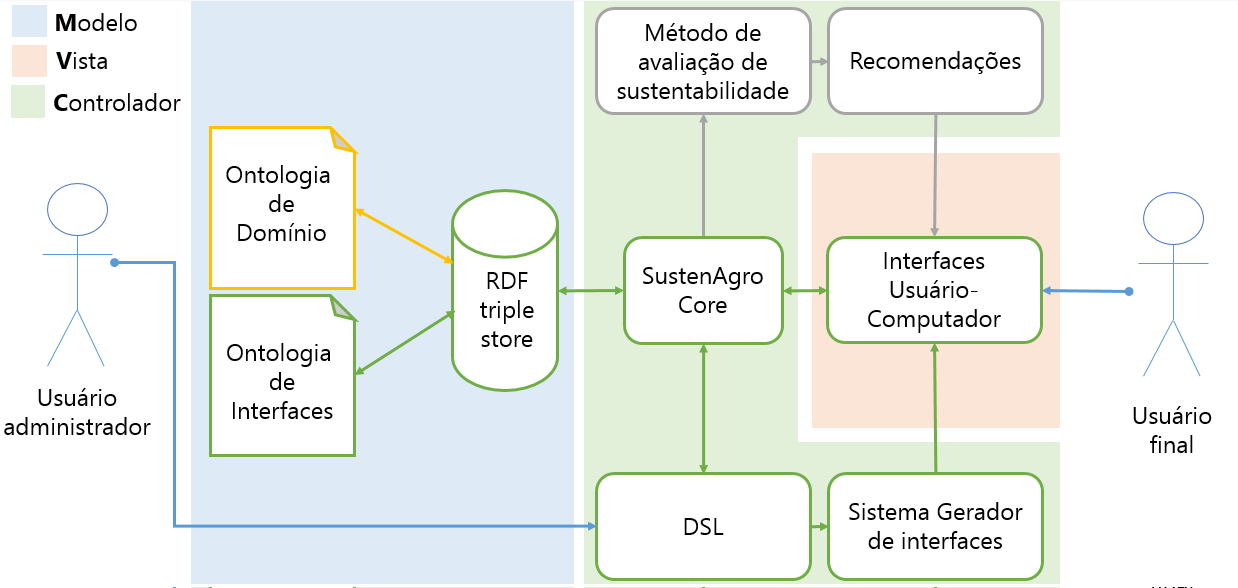
\includegraphics[scale=0.37]{images/Arquitecture}

\caption{Arquitetura do sistema}
\end{figure}


A arquitetura desenvolvida tem duas ontologias base, a ontologia de
dominio dos especialistas que representa o conheçimento sobre sustentabilide
como são os indicadores da sustentabilidade, dimensões da sutentabilidade,
informações geograficas e analyses desenvolvidos, assim como a ontologia
de interfaces de usuario que fornece o suporte de usuários, os datatypes
e o suporte das intefaces graficas.

As ontologias estão instanciadas em uma triplestore que dá suporte
no armazenamento e recuperação das informações para todo o sistema,
o usuário administrador pode configurar o sistema por meio de uma
Domain Specific Language onde são apresentadas as instruções de configuração
na terminologia do especialista, permitindo configurar caracteristicas
do sistema como o dados que compoem um objeto de avaliação, as formulas
da sustentabilidade e as interfaces graficas de resultados.

Permitindo fazer mudanças em qualquer momento da execução do sistema.


\section{Methodology.}

Due to the diversity and the changing nature of the indicators, the
construction of a methodology for the evaluation sustainability and
the requirement to have a massive system of data collection, was necessary
to analyze the technological possibilities to provide an architecture
and information retrieval system to deal with said requirements. It
was decided to implement an information retrieval system based on
triplestore, which needs the development of an ontology.

The development of ontology is responsive type by techniques of rapid
prototyping of coverage and increased complexity, starting with the
most relevant components of the model to the experts and incorporating
each one of the other components by validations, this method was cyclical
obtaining in each prototype cycle.

Among them are the conceptual maps that allow a focused communication
in the field of specialist, in order to represent knowledge of a visual
way and we also have the computational models in semantic web formats
that allow communication with experts in modeling of knowledge.

After having the conceptual model well-defined, modelers represented
this model in OWL standard, after that the expert built questions
that were asked in the system, and it generated the expected results,
then follows a validation phase, integration and adjustment, which
ended with a reliable prototype that represents an ontology sector,
this process will be repeated until you have all sectors of interest
and the required integrity.

The methodology includes the following steps that will represent the
domain knowledge, the process corresponds to a cyclical methodology,
which will be added sectors according to the maturation of the terms
and the need of the information contained:
\begin{enumerate}
\item Definition of entities
\item Definition of ratings
\item Definition of semantic relations
\item Definition the rules and axioms
\item Implementation in OWL
\item Instantiation of individuals
\item Construction of questions
\item Validation through queries
\item Adjustments and integration
\end{enumerate}
This process is not necessarily linear, the modeling can be cyclic
and the modeladors can return to the previous steps as necessary.

The modules that were addressed in the modeling are, in order of development:
\begin{enumerate}
\item Module attributes and data from production plants of sugarcane.
\item Module assessment of sustainability indicators in sugarcane systems.
\item Module representation of sustainability assessment methodology.
\item Module georeferencing connection with the supply of natural resources
data.
\end{enumerate}

\section{Development and Tests}


\subsection{Ontologies}

SustenAgro Ontology represents the critical concepts in the evaluation
of sustainability in the production of sugar cane system in the state
of Sao Paulo, this ontology was developed by a team that includes
specialists in the area of sustainability in agriculture and experts
in semantic web technologies, and tries to represent the system by
means of sustainability indicators, which allow adding, quantify and
simplify information about complex phenomenon so that trends become
more apparent and significant in order to improve the process of understanding
and communication\cite{brandao2002introduccao}. According to \cite{gallopin1996environmental}
the best indicators are those that simplify relevant information,
making them clearer the phenomena.

Indicators of SustenAgro ontology, are classified in three dimensions
standards of sustainability: environmental, social and economic\cite{alkan2009goal};
these dimensions are subdivided into smaller compartments called attributes
for production systems that bring together related identifiers, for
example the environmental dimension has the soil, water and climate
properties.

The dimensions are composed of elements called attributes that classify
each indicators, also have link with the concept of sustainability
value for measure the sustainable of indicators in a given production
system.

In the conceptual map of Figure 2 can be seen a schematic of the main
existing concepts in the ontology developed and how the indicator
element is the center of this model:

\begin{figure}
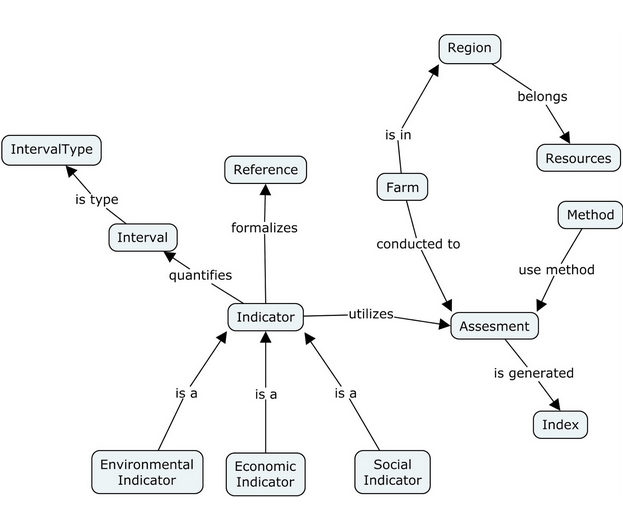
\includegraphics[scale=0.6]{images/PrimeiroMapaConceitual}

\caption{Mapa conceitual da metodologia de desenvolvimento da ontologia}
\end{figure}


The instances of the indicators of ontology will be used by the evaluation
methodology that will generate sustainability indexes, which will
represent the sustainability of the agricultural system evaluated.

According to this methodology, has developed a conceptual map that
represents the concepts and domain relationships and allows communication
with the experts:

The environmental, economic and social dimensions were divided into
attributes and indicators such as presents itself in the following
figures:

Conceptual map of the economic dimension in Figure 3, is important
to know that the production system needs to be sustainable in three
dimensions and not only in one dimension, the economic dimension sometimes
is most analyzed but is not the most important:

\begin{figure}
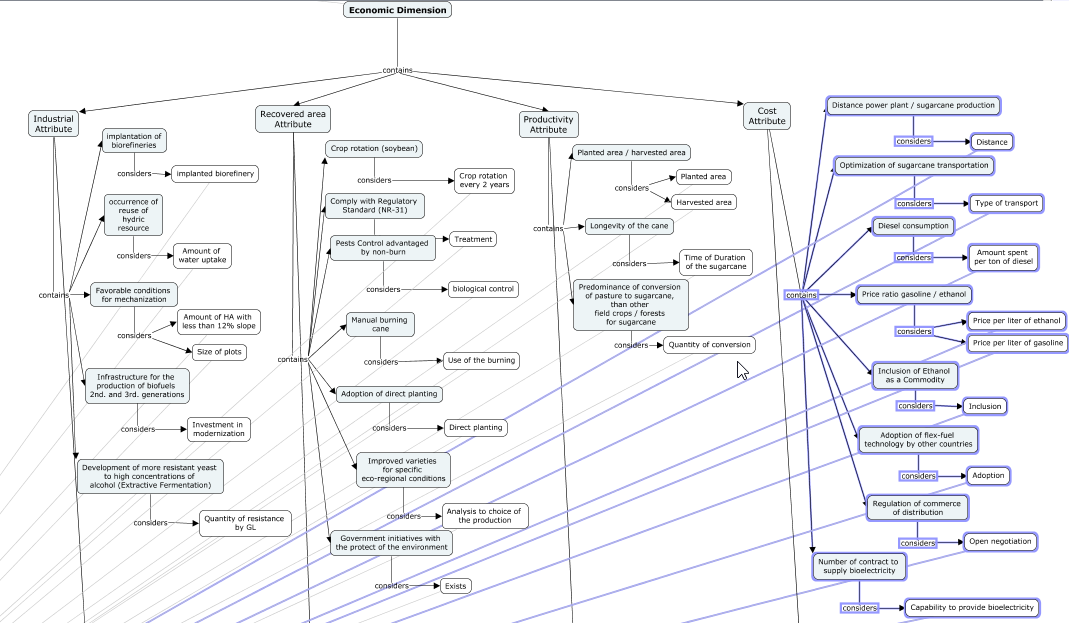
\includegraphics[scale=0.45]{images/DimensaoEconomica}

\caption{Mapa conceitual da Dimensão Econômica}
\end{figure}


Each of these dimensions are linked through the fundamental concepts
of ontologies that are represented in the figure 4.

\begin{figure}
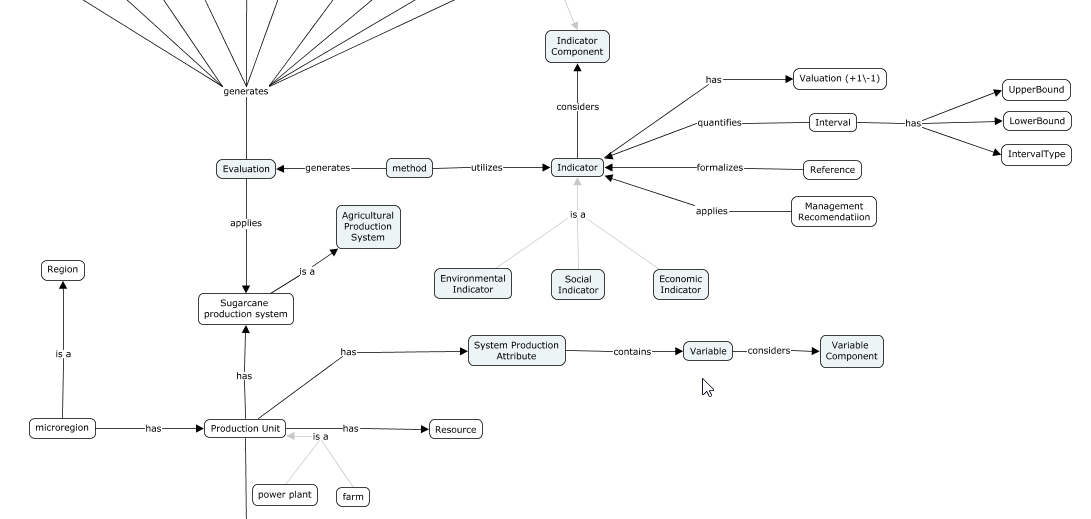
\includegraphics[scale=0.45]{images/PartePrincipal}

\caption{Mapa conceitual dos conceitos fundamentais}
\end{figure}


These elements can generate the sustainability indices and the efficiency
index, that are the output of assessment process.

After modeling the phenomenon through the conceptual map, became a
translation to OWL standard to achieve its interpretation by computers,
the following images show the model made by Protégé tool.

Figure 5 represents the dimension class in Protege:

\begin{figure}
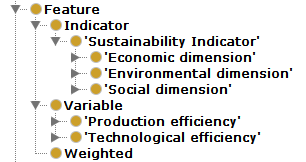
\includegraphics[scale=0.7]{images/Dimensions}

\caption{Classe Dimension}
\end{figure}


Figure 6 represents the attribute class in Protege:

\begin{figure}
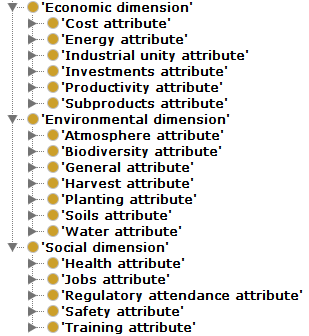
\includegraphics[scale=0.7]{images/Attributes}

\caption{Classe Attribute}
\end{figure}



\subsection{Re-use of ontologies}

Ontologies are formal representations of knowledge that can be reused
according to the needs of each ontological development in the case
of SustenAgro Ontology have consulted sources of ontologies in the
agricultural sector and on the assessment of sustainability, and were
selected two developments the \textquotedbl{}Agricultural ontology
Service \textquotedbl{}which is a model for defining ontologies for
agriculture based on AGROVOC which is a major agricultural vocabularies
developed by FAO, and the ontology of sustainability evaluation ISD-Economics
ontology \cite{brilhante2006information} that provides sustainability
concepts, and according to research it was concluded that there is
an ontology that integrates the concepts of sustainability assessment
in agriculture. These two proposals state of the art will be integrated
into SustenAgro Ontology in the following versions of the ontology,
since the goal of this first version is the identification and definition
of the fundamental concepts of sustainability assessment in the production
of cane sugar system.


\subsection{Domain Specific Language}

A administração das ontologias é realizado por meio de um lenguagen
specifico para uso especialistas em sustenatabilidade que permite
gerenciar os principais conceitos das ontologias para definir o comportamento
deles no processo de calculo dos resultados e na apresentação da interface
grafica, uma visualização deste lenguage é apresentada na figura 7.

\begin{figure}
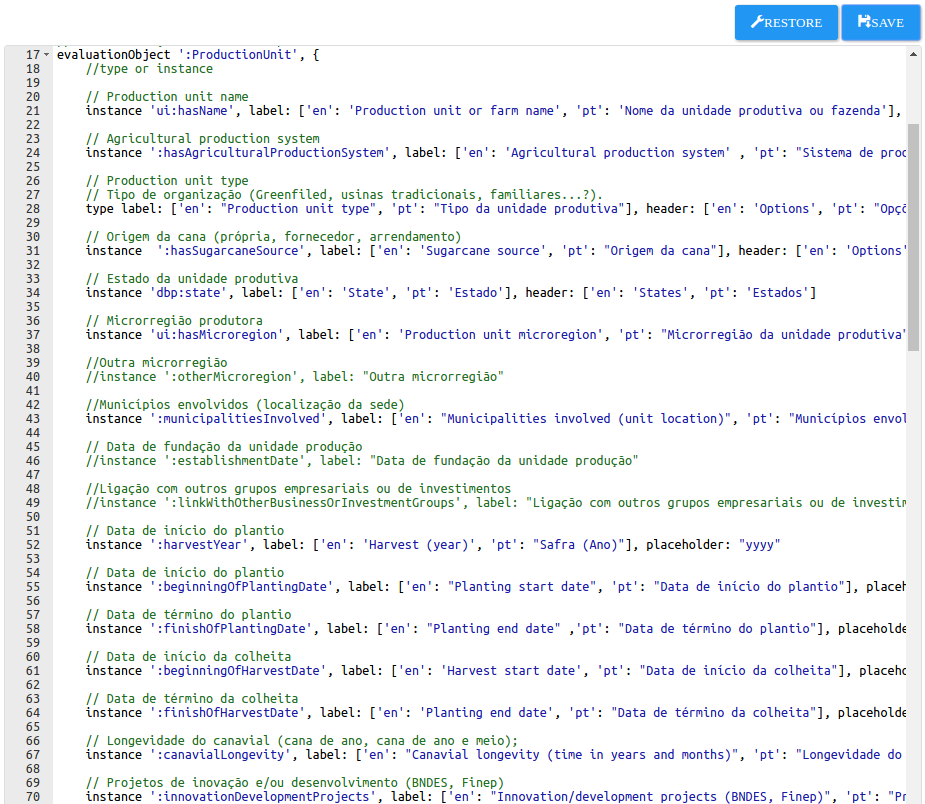
\includegraphics[angle=90,scale=0.4]{images/SustenAgro-dsl-editor}

\caption{SustenAgro domain Specific Language}


\end{figure}



\subsection{SustenAgro Software}

There is a requirement to establish a standard format that define
the terms used in this area, so that people and computer systems that
will use the model have access to the concepts involved. These concepts
are joining the expert knowledge and the knowledge of ontologist to
define a means of communication between stakeholders and computer
systems.

To meet the above requirement was decided to implement the SustenAgro
Ontology through semantic web technologies that enable implement triplestore
information retrieval systems, taking into account these characteristics
was selected the Blazegraph triplestore that supports the SPARQL 1.1
query language.

O sistema desenvolvido foi publicado no endereço web http://java.icmc.usp.br:1300/
como é apresentado na figura 7:

\begin{figure}
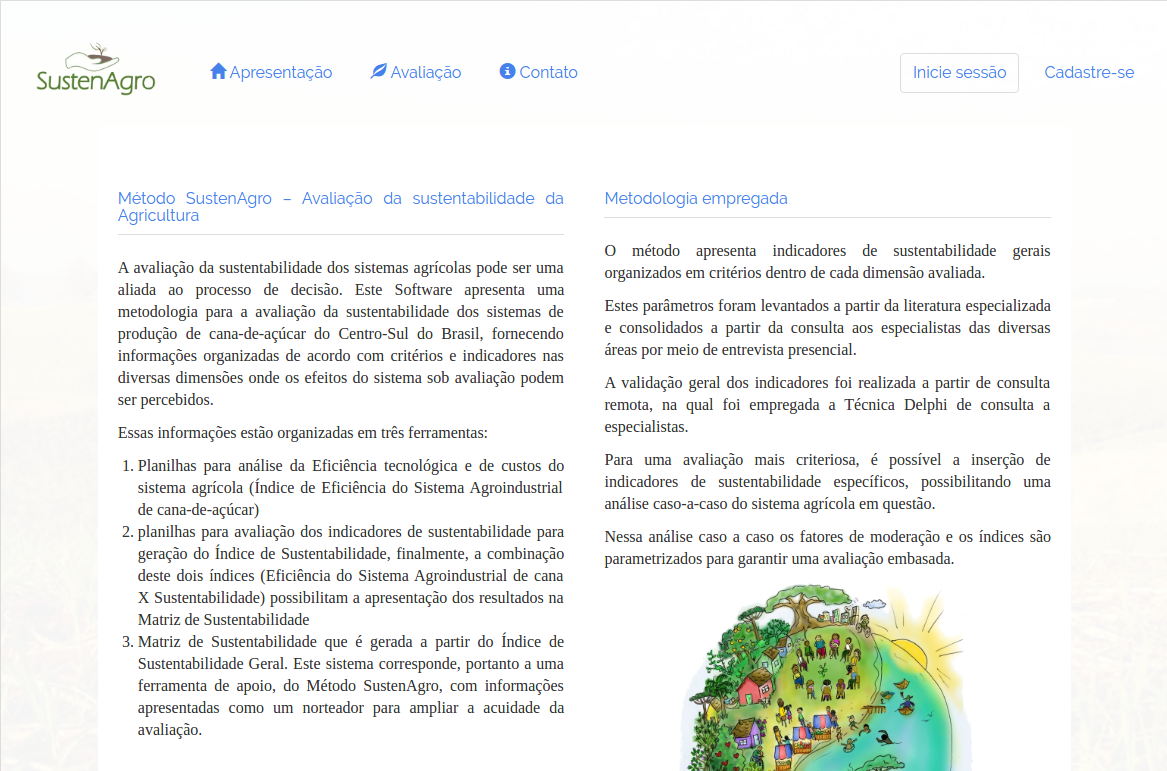
\includegraphics[scale=0.3]{images/SustenAgro-main}

\caption{Tela inicial de sustenagro}
\end{figure}


Nesta tela o usuário pode ver a informação geral do aplicativo, criar
uma nova conta de usuário ou ingresar ao sistema com os dados de usuario.

A partir do ingreso o usuário pode seleccionar o menu avaliação e
escolher entre cadastrar uma nova unidade produtiva ou realizar uma
avaliação de sustentabilidade, como é apresentado na tela da figura
8. 

\begin{figure}
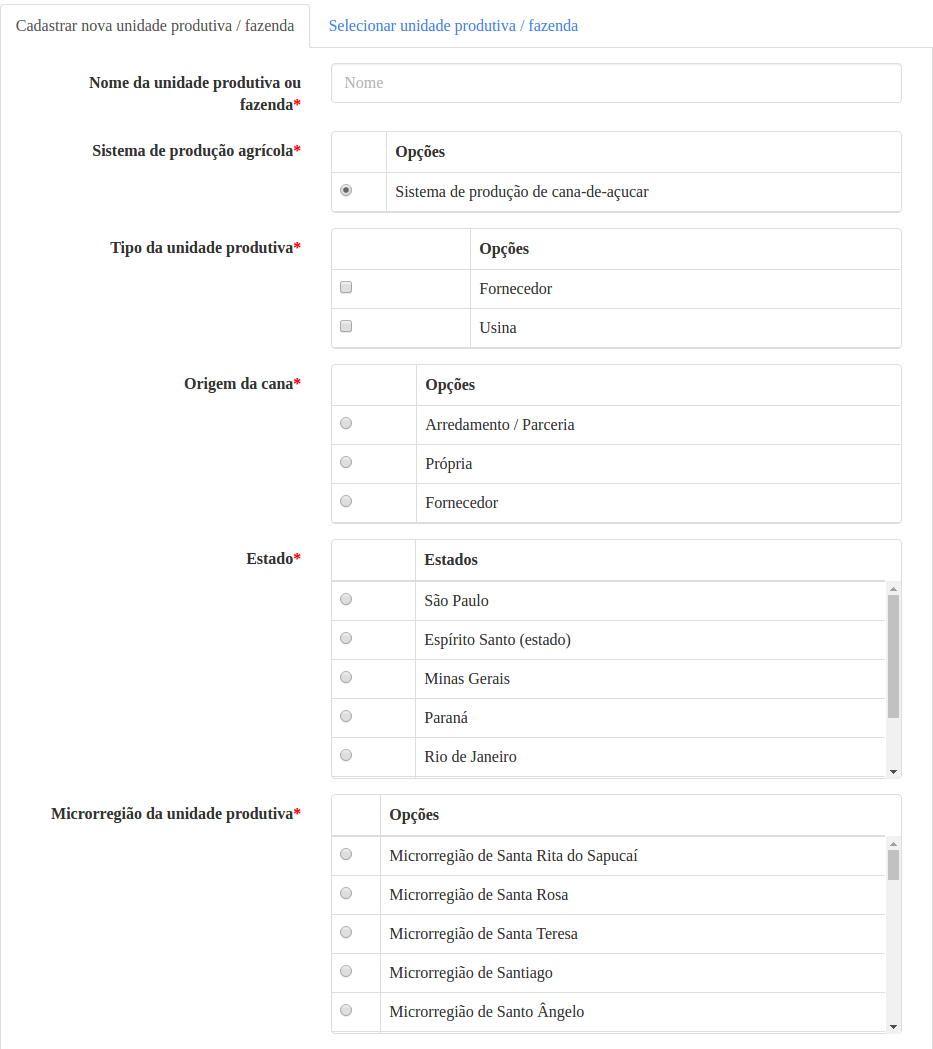
\includegraphics[scale=0.4]{images/SustenAgro-tool}

\caption{Cadastro de nova unidade produtiva/Fazenda}
\end{figure}


Uma vez cadastrada a unidade produtiva/fazenda disponibiliza-se a
opção de criar nova avaliação, ação que vai gerar a tela da figura
9 que permite visualizar as variaveis de eficiencia e os indicadores
para que os usuários preencham cada uma segundo a realidade da unidade
produtiva em avaliação, cada indicador ou variavel de eficiencia tem
varias opções que estão ligadas a valores que quantificam a sustentabilidade,
esses valores estão definidos na ontologia da sustentabilidade e serao
os valores de ingreso para a formula que vai gerar os indices da sustentabilidade.

\begin{figure}
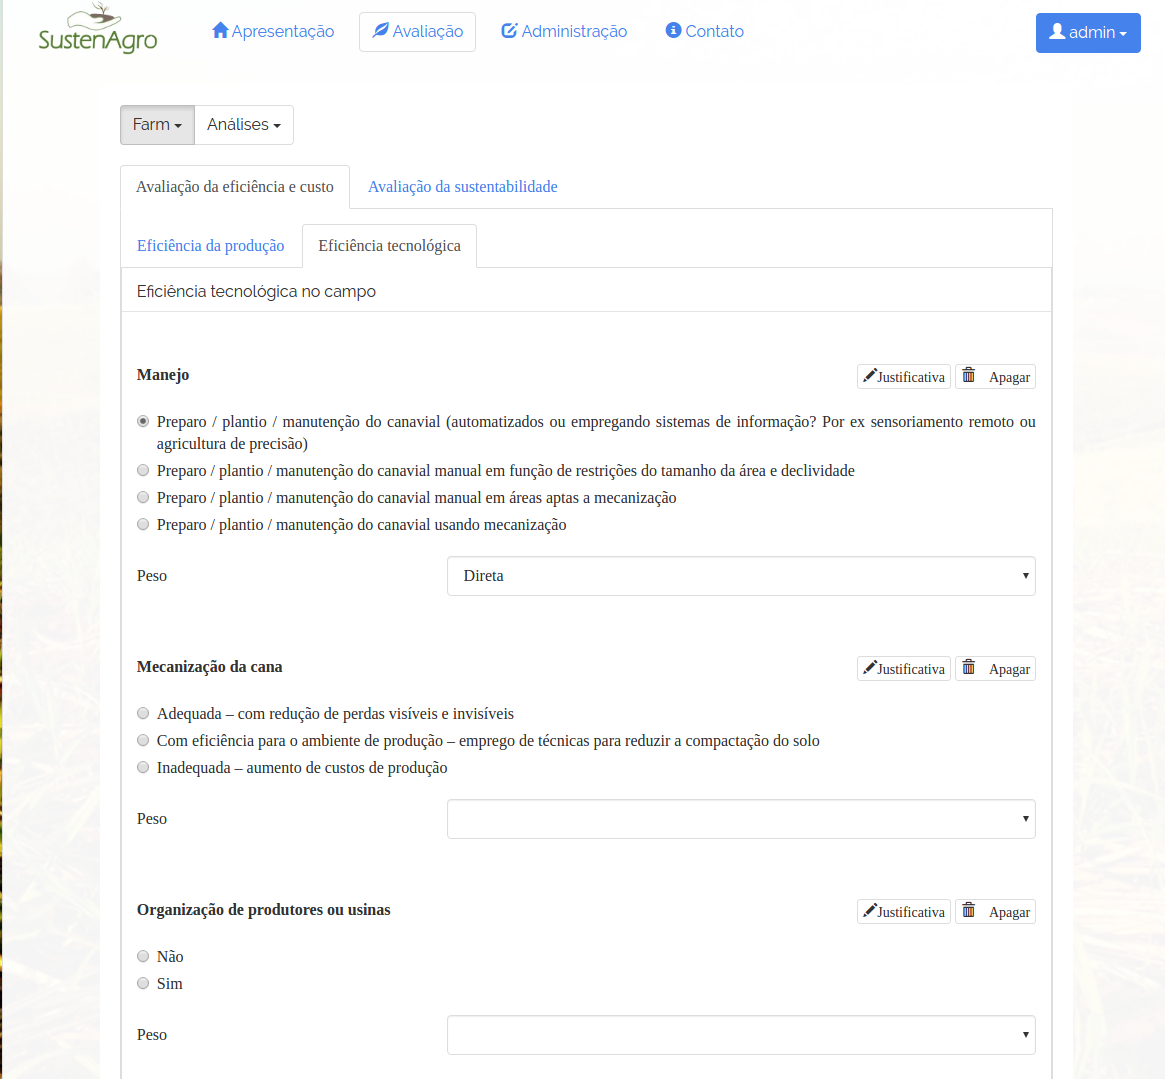
\includegraphics[scale=0.3]{images/SustenAgro-scenario}

\caption{Cadastro das variaveis/indicadores}
\end{figure}


A partir desses desses dados cadastrados são gerados os resultados
do sistema que consistem na planilha de ediciência e custo, na planilha
da sustentabilidade e o relatorio do sistema, as planilhas permitem
a visualizar os atributos das variveis de eficiência e dos indicadores
e a tela de relatorio que apresenta a matrix de avaliação onde são
relaciondas as variaveis de eficiência e de sustentabilidade, o relatio
é apresentado na figura 10.

\begin{figure}
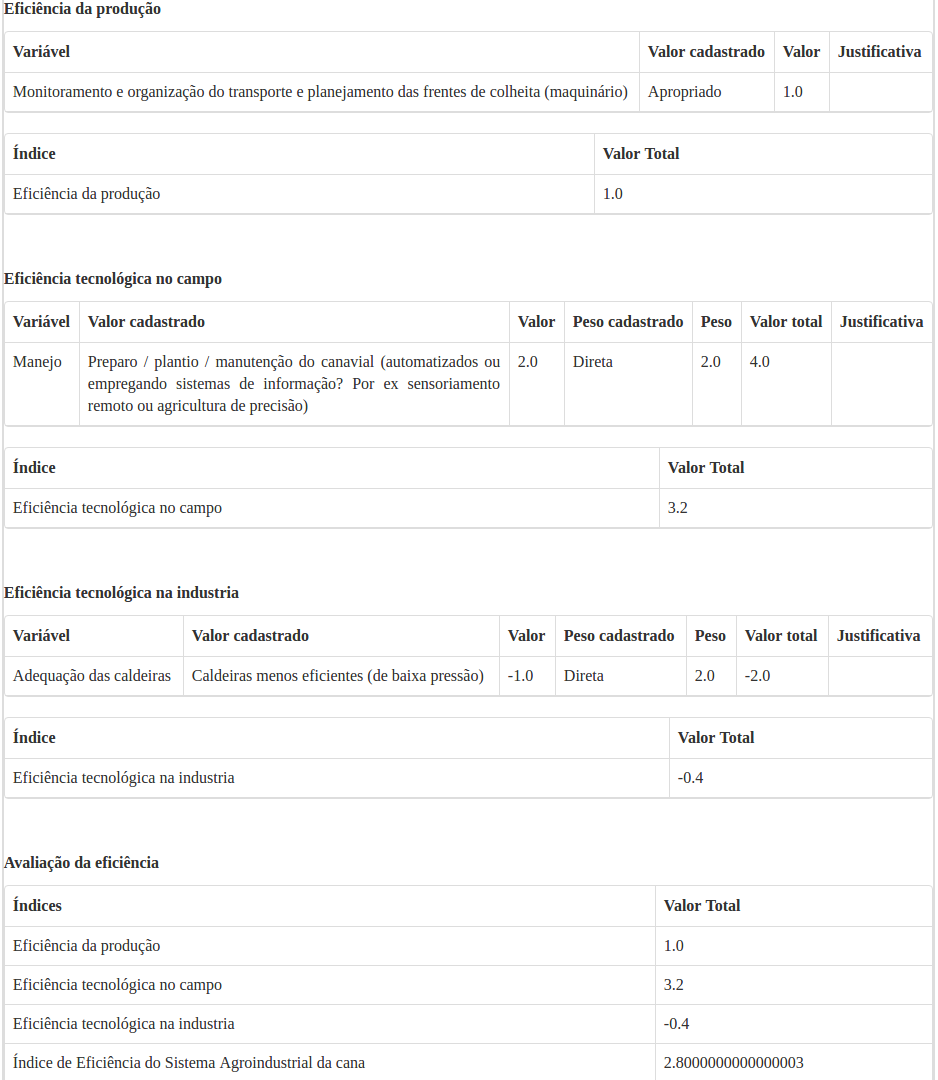
\includegraphics[scale=0.35]{images/SustenAgro-analyses}

\caption{Formato das planilhas de resultado}


\end{figure}



\section{Related work}

Sustainable Development in this context, is the base to serve the
present needs without compromise the future generations to supplement
their needs\cite{brundtland1987our}


\subsection{Agricultural Area}

This part describes the pappers that were relevant to the knowledge
in agriculture.

It is necessary for a standardized ontology using techniques which
make it multilingual so that it can be used without the need for adjustments
to researchers from anywhere.

The papper\cite{lauser2006agrovoc} describes a technique that uses
the AGROVOC multilingual Theasaurus for conversion into an ontology
and also covers the concepts of agriculture that are a focus of the
work, so we analyzed the techniques used to adapt to our ontology.


\subsection{Sustainability Area}

This part describes the pappers that were relevant to the knowledge
in the area of sustainability.

For evaluation of sustainability requires working with indicators
that measure how each practice is sustainable. In the paper\cite{brilhante2006information}
describes an sustainable analysis framework of Amazonas state and
is developed an ontology of these indicators that work in conjunction
with the framework. The last foundation for this work was extremely
important for the development done. Our ontology is based on agricultural
system, the focus on sustainability help to amplify the knowledge
and how to make it computational.

The ontology must be flexible to some extent to accept changes according
to the need of the specialist. The concepts presented by\cite{kraines2011system}
gave an idea of how to make flexible ontology in the area of sustainability
so that it can support new concepts and still not miss the formality
or allow the ambiguous concepts. In this way, we adapt this concepts
and make it in ours.

To describe the sustainability of a clearer and adaptively is important
to understand several indicators that are used in several different
places.\cite{wilson2007contrasting} makes a comparison between sustainability
indicators going through in most of it, analyzing global metrics and
interpreting sustainability among nations, through a clear notion
of sustainability to support knowledge used in the ontology. 


\subsection{Ontologies Area}

In this part of the pappers that were relevant to the knowledge in
the area of development of ontologies in general are described.

For a good ontology is important that the concepts are well defined
and for this and necessary to use techniques to detect semantic conflicts.\cite{alcaraz2010detection}
defines how to assemble senarios in order to detect conflicts or problems
that may have been made in the creation of ontology, the techniques
described can be considered as a kind of reasoning that detects situations
that was not explicit in the ontology. With this and other pappers
related to sustainability we can disambiguate and ensure the concepts
are consistent and follow the expert needs.

For development of an ontology is important to understand the concepts
involved and needs to create an ontology.\cite{wen2007event} describes
about ontologies in computer science and generalized terms that are
needed for development of ontologies, these terms were extremely important
for all stages of creation and analysis of ontology. We do patterns
in links between classes to try make more consistent the ontology.


\subsection{Conceptual basis of ontology}

\cite{brunooliveira2013} was taken as the basis of knowledge and
was chosen by the domain expert. Was taken all the knowledge base
that was used as the indicators and the needs of each and still had
part of integrated sustainability directly with the part of agriculture
geared to the location of the state of São Paulo. It was analyzed
with all the parts described in the dissertation by selecting indicators
previously validated by a group of experts. 


\subsection{Related Technologies}

In order to eliminate ambiguity in semantic understanding and making
mining the relationship between the concepts of knowledge in agriculture,
should be combined with the knowledge among heterogeneous databases.

It proposes a Agricultural Knowledge Grid\cite{cuiping2013agricultural}
which was built with three layers \textquotedbl{}Resource Layer\textquotedbl{},
\textquotedbl{}Semantic Layer\textquotedbl{} and \textquotedbl{}User
Layer\textquotedbl{}, has been applied to \textquotedbl{}Semantic
Extension on Retrieval\textquotedbl{}, \textquotedbl{}Knowledge links\textquotedbl{}
and \textquotedbl{}Experience\textquotedbl{} to deepen \textquotedbl{}Agricultural
Knowledge Services\textquotedbl{}.

AGROVOC is a controlled vocabulary that covers all areas of interest
FAO and consists of 32,000 concepts available in 21 languages, this
tool is used by researchers, librarians and information managers to
index, retrieve and organize data in agricultural information systems.

\cite{lauser2006agrovoc} is an initiative that serves as a reference
in structuring and standardization of agricultural terminology in
multiple languages for use systems in agriculture, the purpose of
this technology is to achieve more interoperability between agricultural
systems.


\section{Results}

Among the results of this research we can emphasize the development
of the conceptual map which established a means of communication between
domain experts and specialists of ontologies, thus achieving the implementation
of the concepts of ontology in computer language.

This approach was chosen because it better fit into the context where
it was being developed. Experts in the field of sustainability had
not domain in ontology development tools and so would be costly teach
them about it, making the conceptual map a more common means of communication
throughout the team and when in the ontology needs experts knowledge
they were introduced the necessary tools.

SustenAgro Ontology is the most relevant results in computational
terms because it allows represent the expert's knowledge in a standard
modeling elements, relations, axioms and rules of the modeled system,
this representation is flexible to change that is needed in this project
since the domain is still in construction also supports information
retrieval technologies.

This ontology was developed using OWL-DL. This was selected because
it is a language created to define ontologies on the Web and also
for a better understanding of the team that developed. Since there
was a need for a data recovery system, it was essential that the ontology
could adapt the semantic web technologies to optimize processes and
adapt to the reality of sustainability.

In addition to the ontology and the conceptual map the ontology was
also adapted into a data recovery system type triplestore, which is
the system used in the semantic web. Was chosen this type of system
because besides the team's expertise in the technology, sustainability
in itself already has some semantic baggage, which introduced into
a scope own optimizes the analysis of sustainable processes and can
communicate with other data systems, providing a greater range of
concepts and analyzes.

This base was made through the triplestore Parliament, this was already
pre-configured on a server facilitating own use. The ontology was
adapted to it and so tests were made based on data collected by experts
to investigate the completeness and consistency of this ontology.

For the evaluation of ontology were made consultations with experts
to create them questions (paths), to answer certain concepts to see
if this ontology was adjusting the nature of the data and that the
very experts expected the ontology.

After this evaluation some adjustments were made to fix some flaws
that had and to generally optimize the ontology. 


\section{Discussion}

One of the difficulties in modeling both the concept map as the ontology
is to reach a consensus of critical concepts, which are the binding
more than one area of expertise, for example in the modeling of the
interface elements as the elements between the indicators and the
assessment methodology, or between the elements of the plant variables
and indicators, this is natural as each expert has a different view
of the phenomenon.

Another difficulty is that the semantic web technologies for knowledge
representation are under development, which leads to incompatibilities
of the various technologies, for example in the development of information
retrieval system there are no software components that facilitate
communication with the server part frameworks. And to validate this
ontology, the experts have some difficult to define how the ontology
have to work in some places to make the validation complete and make
the ontology more reliable at the concepts. 


\section{Conclusions}

In defining the models must define what the purpose of it, which will
guiding each of the discussions that arise when modeling is a complex
phenomenon that can be interpreted in different ways by the experts.

As to the technological development is important to note that the
semantic web storage technologies provide more functionality beyond
the information retrieval, so it is reasonable that the efficiency
is lower in this case is necessary to assess the requirements and
determine the most coherent architecture , which can be hybrid architecture.

Its important to define how the evaluation techniques will be used,
because without a good validation, all of the methods may be invalid
if it’s not have a validation well defined. \textit{(é importante
para definir como serão utilizadas as técnicas de avaliação, porque
sem uma boa validação, todos os métodos podem ser inválidos, se não
é têm uma validação bem definida.) }

\bibliographystyle{plain}
\bibliography{sustenagro}

\end{document}
